\definecolor{Pred}{RGB}{210,55,40}
\definecolor{Qblue}{RGB}{40,120,200}
\definecolor{Wamber}{RGB}{180,120,20}
\definecolor{gridgray}{RGB}{150,150,150}
\definecolor{paneltitle}{RGB}{60,60,60}

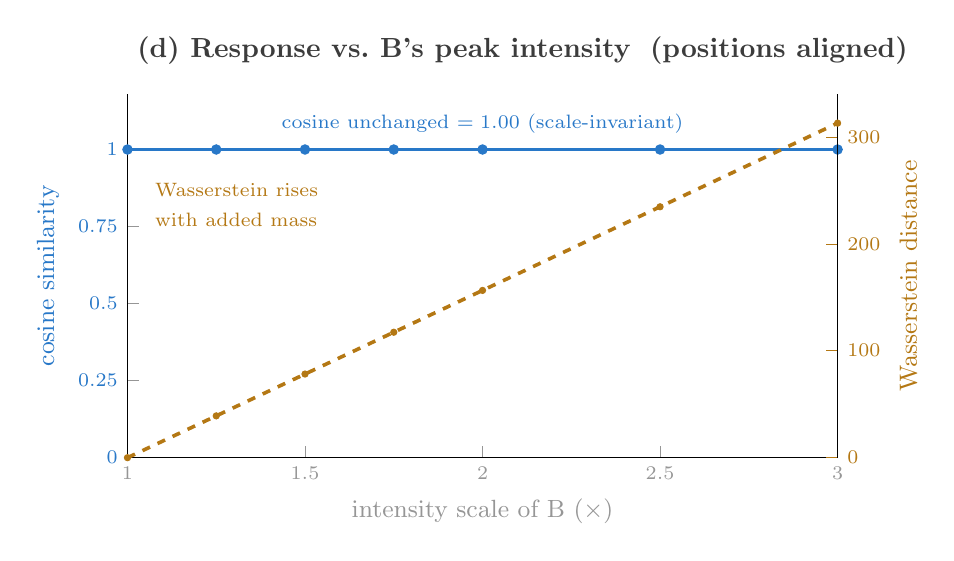
\begin{tikzpicture}

% =====================================================================
% PANEL D — response to scaling B's intensity (peaks aligned)
% =====================================================================
\begin{scope}[shift={(0,0)}]
  \node[anchor=west,paneltitle,font=\bfseries] at (0,0.55)
    {(d) Response vs.\ B's peak intensity \;(positions aligned)};
  \begin{axis}[
      at={(0,0cm)}, anchor=north west,
      width=10.6cm, height=6.2cm,
      xlabel={intensity scale of B ($\times$)},
      xlabel style={font=\small,color=gridgray},
      axis y line*=left, axis x line*=bottom,
      xmin=1, xmax=3, ymin=0, ymax=1.18,
      ylabel={cosine similarity},
      ylabel style={font=\small,color=Qblue},
      ytick={0,0.25,0.5,0.75,1.0},
      yticklabel style={color=Qblue,font=\scriptsize},
      xtick={1,1.5,2,2.5,3},
      xticklabel style={color=gridgray,font=\scriptsize},
      tick style={color=gridgray},
    ]
    % cosine: flat at 1.0 regardless of intensity scale
    \addplot[Qblue,line width=1.3pt,mark=*,mark size=1.2pt] coordinates {
      (1,1)(1.25,1)(1.5,1)(1.75,1)(2,1)(2.5,1)(3,1)};
    \node[Qblue,font=\scriptsize,anchor=south] at (axis cs:2,1.02)
      {cosine unchanged $=1.00$ (scale-invariant)};
  \end{axis}
  \begin{axis}[
      at={(0,0cm)}, anchor=north west,
      width=10.6cm, height=6.2cm,
      axis y line*=right, axis x line=none,
      xmin=1, xmax=3, ymin=0, ymax=340,
      ylabel={Wasserstein distance},
      ylabel style={font=\small,color=Wamber},
      ytick={0,100,200,300},
      yticklabel style={color=Wamber,font=\scriptsize},
      tick style={color=Wamber},
    ]
    % Wasserstein grows linearly with added mass
    \addplot[Wamber,line width=1.3pt,dashed] coordinates {(1,0)(3,312.8)};
    \addplot[Wamber,only marks,mark=*,mark size=1.1pt] coordinates {
      (1,0)(1.25,39.1)(1.5,78.2)(1.75,117.3)(2,156.4)(2.5,234.6)(3,312.8)};
    \node[Wamber,font=\scriptsize,anchor=west] at (axis cs:1.05,250)
      {Wasserstein rises};
    \node[Wamber,font=\scriptsize,anchor=west] at (axis cs:1.05,222)
      {with added mass};
  \end{axis}
\end{scope}

\end{tikzpicture}
